
%% bare_jrnl.tex
%% V1.3
%% 2007/01/11
%% by Michael Shell
%% see http://www.michaelshell.org/
%% for current contact information.
%%
%% This is a skeleton file demonstrating the use of IEEEtran.cls
%% (requires IEEEtran.cls version 1.7 or later) with an IEEE journal paper.
%%
%% Support sites:
%% http://www.michaelshell.org/tex/ieeetran/
%% http://www.ctan.org/tex-archive/macros/latex/contrib/IEEEtran/
%% and
%% http://www.ieee.org/



% *** Authors should verify (and, if needed, correct) their LaTeX system  ***
% *** with the testflow diagnostic prior to trusting their LaTeX platform ***
% *** with production work. IEEE's font choices can trigger bugs that do  ***
% *** not appear when using other class files.                            ***
% The testflow support page is at:
% http://www.michaelshell.org/tex/testflow/


%%*************************************************************************
%% Legal Notice:
%% This code is offered as-is without any warranty either expressed or
%% implied; without even the implied warranty of MERCHANTABILITY or
%% FITNESS FOR A PARTICULAR PURPOSE! 
%% User assumes all risk.
%% In no event shall IEEE or any contributor to this code be liable for
%% any damages or losses, including, but not limited to, incidental,
%% consequential, or any other damages, resulting from the use or misuse
%% of any information contained here.
%%
%% All comments are the opinions of their respective authors and are not
%% necessarily endorsed by the IEEE.
%%
%% This work is distributed under the LaTeX Project Public License (LPPL)
%% ( http://www.latex-project.org/ ) version 1.3, and may be freely used,
%% distributed and modified. A copy of the LPPL, version 1.3, is included
%% in the base LaTeX documentation of all distributions of LaTeX released
%% 2003/12/01 or later.
%% Retain all contribution notices and credits.
%% ** Modified files should be clearly indicated as such, including  **
%% ** renaming them and changing author support contact information. **
%%
%% File list of work: IEEEtran.cls, IEEEtran_HOWTO.pdf, bare_adv.tex,
%%                    bare_conf.tex, bare_jrnl.tex, bare_jrnl_compsoc.tex
%%*************************************************************************

% Note that the a4paper option is mainly intended so that authors in
% countries using A4 can easily print to A4 and see how their papers will
% look in print - the typesetting of the document will not typically be
% affected with changes in paper size (but the bottom and side margins will).
% Use the testflow package mentioned above to verify correct handling of
% both paper sizes by the user's LaTeX system.
%
% Also note that the "draftcls" or "draftclsnofoot", not "draft", option
% should be used if it is desired that the figures are to be displayed in
% draft mode.
%
\documentclass[journal]{IEEEtran}
%
% If IEEEtran.cls has not been installed into the LaTeX system files,
% manually specify the path to it like:
% \documentclass[journal]{../sty/IEEEtran}

\usepackage{url}
\usepackage{pgfplots}  % Used to produce graphs.
\usepackage{pgfplotstable} % Used to make graphs from reading tables.
\usepackage{datatool}  % Used to read CSV and make simple table.
\usepackage{listings}  % Show source code.
\usepackage{algorithm}% http://ctan.org/pkg/algorithms
\usepackage{algpseudocode}% http://ctan.org/pkg/algorithmicx


% Some very useful LaTeX packages include:
% (uncomment the ones you want to load)


% *** MISC UTILITY PACKAGES ***
%
%\usepackage{ifpdf}
% Heiko Oberdiek's ifpdf.sty is very useful if you need conditional
% compilation based on whether the output is pdf or dvi.
% usage:
% \ifpdf
%   % pdf code
% \else
%   % dvi code
% \fi
% The latest version of ifpdf.sty can be obtained from:
% http://www.ctan.org/tex-archive/macros/latex/contrib/oberdiek/
% Also, note that IEEEtran.cls V1.7 and later provides a builtin
% \ifCLASSINFOpdf conditional that works the same way.
% When switching from latex to pdflatex and vice-versa, the compiler may
% have to be run twice to clear warning/error messages.


% *** SOURCE CODE (LISTINGS) SETUP ***
\lstloadlanguages{C++} % Load Perl syntax for listings, for a list of other languages supported see: ftp://ftp.tex.ac.uk/tex-archive/macros/latex/contrib/listings/listings.pdf
\lstset{language=C++, % Use Perl in this example
        frame=single, % Single frame around code
        basicstyle=\small\ttfamily, % Use small true type font
        identifierstyle=, % Nothing special about identifiers                                         
        commentstyle=\usefont{T1}{pcr}{m}{sl}\color{MyDarkGreen}\small, % Comments small dark green courier font
        showstringspaces=false, % Don't put marks in string spaces
        tabsize=4, % 4 spaces per tab
        %
        numbers=left, % Line numbers on left
        firstnumber=1, % Line numbers start with line 1
        stepnumber=5, % Line numbers go in steps of 5
        breaklines=true,
        float=*, % Make listing span both columns.
        lineskip=-1ex % Make the list listings single spaced by undoing 2x spacing
}

\newcommand{\cppcode}[2]{
\begin{figure*}
\lstinputlisting[language=C++,caption=#2,label=#1]{#1.cpp}
\end{figure*}
}

\newcommand{\hppcode}[2]{
\begin{figure*}
\lstinputlisting[language=C++,caption=#2,label=#1]{#1.hpp}
\end{figure*}
}

\newcommand{\bashout}[2]{
\begin{figure*}
\lstinputlisting[language=bash,caption=#2,label=#1]{#1.out}
\end{figure*}
}



% *** CITATION PACKAGES ***
%
%\usepackage{cite}
% cite.sty was written by Donald Arseneau
% V1.6 and later of IEEEtran pre-defines the format of the cite.sty package
% \cite{} output to follow that of IEEE. Loading the cite package will
% result in citation numbers being automatically sorted and properly
% "compressed/ranged". e.g., [1], [9], [2], [7], [5], [6] without using
% cite.sty will become [1], [2], [5]--[7], [9] using cite.sty. cite.sty's
% \cite will automatically add leading space, if needed. Use cite.sty's
% noadjust option (cite.sty V3.8 and later) if you want to turn this off.
% cite.sty is already installed on most LaTeX systems. Be sure and use
% version 4.0 (2003-05-27) and later if using hyperref.sty. cite.sty does
% not currently provide for hyperlinked citations.
% The latest version can be obtained at:
% http://www.ctan.org/tex-archive/macros/latex/contrib/cite/
% The documentation is contained in the cite.sty file itself.






% *** GRAPHICS RELATED PACKAGES ***
%
\ifCLASSINFOpdf
  % \usepackage[pdftex]{graphicx}
  % declare the path(s) where your graphic files are
  % \graphicspath{{../pdf/}{../jpeg/}}
  % and their extensions so you won't have to specify these with
  % every instance of \includegraphics
  % \DeclareGraphicsExtensions{.pdf,.jpeg,.png}
\else
  % or other class option (dvipsone, dvipdf, if not using dvips). graphicx
  % will default to the driver specified in the system graphics.cfg if no
  % driver is specified.
  % \usepackage[dvips]{graphicx}
  % declare the path(s) where your graphic files are
  % \graphicspath{{../eps/}}
  % and their extensions so you won't have to specify these with
  % every instance of \includegraphics
  % \DeclareGraphicsExtensions{.eps}
\fi
% graphicx was written by David Carlisle and Sebastian Rahtz. It is
% required if you want graphics, photos, etc. graphicx.sty is already
% installed on most LaTeX systems. The latest version and documentation can
% be obtained at: 
% http://www.ctan.org/tex-archive/macros/latex/required/graphics/
% Another good source of documentation is "Using Imported Graphics in
% LaTeX2e" by Keith Reckdahl which can be found as epslatex.ps or
% epslatex.pdf at: http://www.ctan.org/tex-archive/info/
%
% latex, and pdflatex in dvi mode, support graphics in encapsulated
% postscript (.eps) format. pdflatex in pdf mode supports graphics
% in .pdf, .jpeg, .png and .mps (metapost) formats. Users should ensure
% that all non-photo figures use a vector format (.eps, .pdf, .mps) and
% not a bitmapped formats (.jpeg, .png). IEEE frowns on bitmapped formats
% which can result in "jaggedy"/blurry rendering of lines and letters as
% well as large increases in file sizes.
%
% You can find documentation about the pdfTeX application at:
% http://www.tug.org/applications/pdftex





% *** MATH PACKAGES ***
%
%\usepackage[cmex10]{amsmath}
% A popular package from the American Mathematical Society that provides
% many useful and powerful commands for dealing with mathematics. If using
% it, be sure to load this package with the cmex10 option to ensure that
% only type 1 fonts will utilized at all point sizes. Without this option,
% it is possible that some math symbols, particularly those within
% footnotes, will be rendered in bitmap form which will result in a
% document that can not be IEEE Xplore compliant!
%
% Also, note that the amsmath package sets \interdisplaylinepenalty to 10000
% thus preventing page breaks from occurring within multiline equations. Use:
%\interdisplaylinepenalty=2500
% after loading amsmath to restore such page breaks as IEEEtran.cls normally
% does. amsmath.sty is already installed on most LaTeX systems. The latest
% version and documentation can be obtained at:
% http://www.ctan.org/tex-archive/macros/latex/required/amslatex/math/





% *** SPECIALIZED LIST PACKAGES ***
%
%\usepackage{algorithmic}
% algorithmic.sty was written by Peter Williams and Rogerio Brito.
% This package provides an algorithmic environment fo describing algorithms.
% You can use the algorithmic environment in-text or within a figure
% environment to provide for a floating algorithm. Do NOT use the algorithm
% floating environment provided by algorithm.sty (by the same authors) or
% algorithm2e.sty (by Christophe Fiorio) as IEEE does not use dedicated
% algorithm float types and packages that provide these will not provide
% correct IEEE style captions. The latest version and documentation of
% algorithmic.sty can be obtained at:
% http://www.ctan.org/tex-archive/macros/latex/contrib/algorithms/
% There is also a support site at:
% http://algorithms.berlios.de/index.html
% Also of interest may be the (relatively newer and more customizable)
% algorithmicx.sty package by Szasz Janos:
% http://www.ctan.org/tex-archive/macros/latex/contrib/algorithmicx/




% *** ALIGNMENT PACKAGES ***
%
%\usepackage{array}
% Frank Mittelbach's and David Carlisle's array.sty patches and improves
% the standard LaTeX2e array and tabular environments to provide better
% appearance and additional user controls. As the default LaTeX2e table
% generation code is lacking to the point of almost being broken with
% respect to the quality of the end results, all users are strongly
% advised to use an enhanced (at the very least that provided by array.sty)
% set of table tools. array.sty is already installed on most systems. The
% latest version and documentation can be obtained at:
% http://www.ctan.org/tex-archive/macros/latex/required/tools/


%\usepackage{mdwmath}
%\usepackage{mdwtab}
% Also highly recommended is Mark Wooding's extremely powerful MDW tools,
% especially mdwmath.sty and mdwtab.sty which are used to format equations
% and tables, respectively. The MDWtools set is already installed on most
% LaTeX systems. The lastest version and documentation is available at:
% http://www.ctan.org/tex-archive/macros/latex/contrib/mdwtools/


% IEEEtran contains the IEEEeqnarray family of commands that can be used to
% generate multiline equations as well as matrices, tables, etc., of high
% quality.


%\usepackage{eqparbox}
% Also of notable interest is Scott Pakin's eqparbox package for creating
% (automatically sized) equal width boxes - aka "natural width parboxes".
% Available at:
% http://www.ctan.org/tex-archive/macros/latex/contrib/eqparbox/





% *** SUBFIGURE PACKAGES ***
%\usepackage[tight,footnotesize]{subfigure}
% subfigure.sty was written by Steven Douglas Cochran. This package makes it
% easy to put subfigures in your figures. e.g., "Figure 1a and 1b". For IEEE
% work, it is a good idea to load it with the tight package option to reduce
% the amount of white space around the subfigures. subfigure.sty is already
% installed on most LaTeX systems. The latest version and documentation can
% be obtained at:
% http://www.ctan.org/tex-archive/obsolete/macros/latex/contrib/subfigure/
% subfigure.sty has been superceeded by subfig.sty.



%\usepackage[caption=false]{caption}
%\usepackage[font=footnotesize]{subfig}
% subfig.sty, also written by Steven Douglas Cochran, is the modern
% replacement for subfigure.sty. However, subfig.sty requires and
% automatically loads Axel Sommerfeldt's caption.sty which will override
% IEEEtran.cls handling of captions and this will result in nonIEEE style
% figure/table captions. To prevent this problem, be sure and preload
% caption.sty with its "caption=false" package option. This is will preserve
% IEEEtran.cls handing of captions. Version 1.3 (2005/06/28) and later 
% (recommended due to many improvements over 1.2) of subfig.sty supports
% the caption=false option directly:
%\usepackage[caption=false,font=footnotesize]{subfig}
%
% The latest version and documentation can be obtained at:
% http://www.ctan.org/tex-archive/macros/latex/contrib/subfig/
% The latest version and documentation of caption.sty can be obtained at:
% http://www.ctan.org/tex-archive/macros/latex/contrib/caption/




% *** FLOAT PACKAGES ***
%
%\usepackage{fixltx2e}
% fixltx2e, the successor to the earlier fix2col.sty, was written by
% Frank Mittelbach and David Carlisle. This package corrects a few problems
% in the LaTeX2e kernel, the most notable of which is that in current
% LaTeX2e releases, the ordering of single and double column floats is not
% guaranteed to be preserved. Thus, an unpatched LaTeX2e can allow a
% single column figure to be placed prior to an earlier double column
% figure. The latest version and documentation can be found at:
% http://www.ctan.org/tex-archive/macros/latex/base/



%\usepackage{stfloats}
% stfloats.sty was written by Sigitas Tolusis. This package gives LaTeX2e
% the ability to do double column floats at the bottom of the page as well
% as the top. (e.g., "\begin{figure*}[!b]" is not normally possible in
% LaTeX2e). It also provides a command:
%\fnbelowfloat
% to enable the placement of footnotes below bottom floats (the standard
% LaTeX2e kernel puts them above bottom floats). This is an invasive package
% which rewrites many portions of the LaTeX2e float routines. It may not work
% with other packages that modify the LaTeX2e float routines. The latest
% version and documentation can be obtained at:
% http://www.ctan.org/tex-archive/macros/latex/contrib/sttools/
% Documentation is contained in the stfloats.sty comments as well as in the
% presfull.pdf file. Do not use the stfloats baselinefloat ability as IEEE
% does not allow \baselineskip to stretch. Authors submitting work to the
% IEEE should note that IEEE rarely uses double column equations and
% that authors should try to avoid such use. Do not be tempted to use the
% cuted.sty or midfloat.sty packages (also by Sigitas Tolusis) as IEEE does
% not format its papers in such ways.


%\ifCLASSOPTIONcaptionsoff
%  \usepackage[nomarkers]{endfloat}
% \let\MYoriglatexcaption\caption
% \renewcommand{\caption}[2][\relax]{\MYoriglatexcaption[#2]{#2}}
%\fi
% endfloat.sty was written by James Darrell McCauley and Jeff Goldberg.
% This package may be useful when used in conjunction with IEEEtran.cls'
% captionsoff option. Some IEEE journals/societies require that submissions
% have lists of figures/tables at the end of the paper and that
% figures/tables without any captions are placed on a page by themselves at
% the end of the document. If needed, the draftcls IEEEtran class option or
% \CLASSINPUTbaselinestretch interface can be used to increase the line
% spacing as well. Be sure and use the nomarkers option of endfloat to
% prevent endfloat from "marking" where the figures would have been placed
% in the text. The two hack lines of code above are a slight modification of
% that suggested by in the endfloat docs (section 8.3.1) to ensure that
% the full captions always appear in the list of figures/tables - even if
% the user used the short optional argument of \caption[]{}.
% IEEE papers do not typically make use of \caption[]'s optional argument,
% so this should not be an issue. A similar trick can be used to disable
% captions of packages such as subfig.sty that lack options to turn off
% the subcaptions:
% For subfig.sty:
% \let\MYorigsubfloat\subfloat
% \renewcommand{\subfloat}[2][\relax]{\MYorigsubfloat[]{#2}}
% For subfigure.sty:
% \let\MYorigsubfigure\subfigure
% \renewcommand{\subfigure}[2][\relax]{\MYorigsubfigure[]{#2}}
% However, the above trick will not work if both optional arguments of
% the \subfloat/subfig command are used. Furthermore, there needs to be a
% description of each subfigure *somewhere* and endfloat does not add
% subfigure captions to its list of figures. Thus, the best approach is to
% avoid the use of subfigure captions (many IEEE journals avoid them anyway)
% and instead reference/explain all the subfigures within the main caption.
% The latest version of endfloat.sty and its documentation can obtained at:
% http://www.ctan.org/tex-archive/macros/latex/contrib/endfloat/
%
% The IEEEtran \ifCLASSOPTIONcaptionsoff conditional can also be used
% later in the document, say, to conditionally put the References on a 
% page by themselves.





% *** PDF, URL AND HYPERLINK PACKAGES ***
%
%\usepackage{url}
% url.sty was written by Donald Arseneau. It provides better support for
% handling and breaking URLs. url.sty is already installed on most LaTeX
% systems. The latest version can be obtained at:
% http://www.ctan.org/tex-archive/macros/latex/contrib/misc/
% Read the url.sty source comments for usage information. Basically,
% \url{my_url_here}.





% *** Do not adjust lengths that control margins, column widths, etc. ***
% *** Do not use packages that alter fonts (such as pslatex).         ***
% There should be no need to do such things with IEEEtran.cls V1.6 and later.
% (Unless specifically asked to do so by the journal or conference you plan
% to submit to, of course. )


% correct bad hyphenation here
\hyphenation{op-tical net-works semi-conduc-tor}

\linespread{2}
\begin{document}
%
% paper title
% can use linebreaks \\ within to get better formatting as desired
\title{Laser Patroll Final Report}
%
%
% author names and IEEE memberships
% note positions of commas and nonbreaking spaces ( ~ ) LaTeX will not break
% a structure at a ~ so this keeps an author's name from being broken across
% two lines.
% use \thanks{} to gain access to the first footnote area
% a separate \thanks must be used for each paragraph as LaTeX2e's \thanks
% was not built to handle multiple paragraphs
%

\author{Eric~Krause,~\IEEEmembership{Griddle~Master,~Breakfast~Confectionery~Guild,}
        Josh~Moles,~\IEEEmembership{Waffle~Stomper,~Breakfast~Confectionery~Guild,}
        and~Erik~Rhodes,~\IEEEmembership{Eggtravagent~Chef,~Breakfast~Confectionery~Guild}% <-this % stops a space
\thanks{E. Krause is a master of the arts of pancake capture at the Guild.}% <-this % stops a space
\thanks{J. Moles enjoys the art of waffle design.}% <-this % stops a space
\thanks{E. Rhodes does not understand why eggs are not more common in everyone's daily life.}%
\thanks{Manuscript completed for 10 December 2013.}}

% note the % following the last \IEEEmembership and also \thanks - 
% these prevent an unwanted space from occurring between the last author name
% and the end of the author line. i.e., if you had this:
% 
% \author{....lastname \thanks{...} \thanks{...} }
%                     ^------------^------------^----Do not want these spaces!
%
% a space would be appended to the last name and could cause every name on that
% line to be shifted left slightly. This is one of those "LaTeX things". For
% instance, "\textbf{A} \textbf{B}" will typeset as "A B" not "AB". To get
% "AB" then you have to do: "\textbf{A}\textbf{B}"
% \thanks is no different in this regard, so shield the last } of each \thanks
% that ends a line with a % and do not let a space in before the next \thanks.
% Spaces after \IEEEmembership other than the last one are OK (and needed) as
% you are supposed to have spaces between the names. For what it is worth,
% this is a minor point as most people would not even notice if the said evil
% space somehow managed to creep in.



% The paper headers
\markboth{Journal of Doctor Robotnik Baking through Sorting,~Vol.~19,No.~2, December~2013}%
{Shell \MakeLowercase{\textit{et al.}}: Bare Demo of IEEEtran.cls for Journals}
% The only time the second header will appear is for the odd numbered pages
% after the title page when using the twoside option.
% 
% *** Note that you probably will NOT want to include the author's ***
% *** name in the headers of peer review papers.                   ***
% You can use \ifCLASSOPTIONpeerreview for conditional compilation here if
% you desire.




% If you want to put a publisher's ID mark on the page you can do it like
% this:
%\IEEEpubid{0000--0000/00\$00.00~\copyright~2007 IEEE}
% Remember, if you use this you must call \IEEEpubidadjcol in the second
% column for its text to clear the IEEEpubid mark.



% use for special paper notices
%\IEEEspecialpapernotice{(Invited Paper)}




% make the title area
\maketitle


\begin{abstract}
%\boldmath
%TODO: Abstract needs expanding once paper is completed.
This work discusses a benchmarking of four sort algorithms tested against each other for a Portland State University ECE 588 project. The four sorts tested were C++'s \texttt{std::sort}, Quicksort, Merge sort, and Bitonic sort.
\end{abstract}
% IEEEtran.cls defaults to using nonbold math in the Abstract.
% This preserves the distinction between vectors and scalars. However,
% if the journal you are submitting to favors bold math in the abstract,
% then you can use LaTeX's standard command \boldmath at the very start
% of the abstract to achieve this. Many IEEE journals frown on math
% in the abstract anyway.

% Note that keywords are not normally used for peerreview papers.
\begin{IEEEkeywords}
soting, Bitonic sort, Quicksort, Merge sort, class.
\end{IEEEkeywords}






% For peer review papers, you can put extra information on the cover
% page as needed:
% \ifCLASSOPTIONpeerreview
% \begin{center} \bfseries EDICS Category: 3-BBND \end{center}
% \fi
%
% For peerreview papers, this IEEEtran command inserts a page break and
% creates the second title. It will be ignored for other modes.
\IEEEpeerreviewmaketitle



\section{Introduction}
% The very first letter is a 2 line initial drop letter followed
% by the rest of the first word in caps.
% 
% form to use if the first word consists of a single letter:
% \IEEEPARstart{A}{demo} file is ....
% 
% form to use if you need the single drop letter followed by
% normal text (unknown if ever used by IEEE):
% \IEEEPARstart{A}{}demo file is ....
% 
% Some journals put the first two words in caps:
% \IEEEPARstart{T}{his demo} file is ....
% 
% Here we have the typical use of a "T" for an initial drop letter
% and "HIS" in caps to complete the first word.

% TODO: Probably want to expand this intro.
\IEEEPARstart{S}{orting} data is a task in computer science that is highly important because it is a very common operation. This report discusses the work done by Laser Patroll [sic] for a team project at Portland State University for the ECE 588 course taught in Fall 2013. The focus of this project was twofold: 
\begin{itemize}
\item First, to either identify parallel sorting algorithms and implement them, or parallelize existing serial (single-threaded) algorithms. 
\item Second, benchmark each of the selected algorithms against each other.  This involved sorting lists of varying lengths using varying numbers of threads, while measuring the relative performance and behavior of the selected algorithms against a known, highly optimized sort, the C++ \texttt{std::sort}.
\end{itemize}


The four algorithms benchmarked and discussed in this report are the C++ \texttt{std::sort}, Quicksort~\cite{Hoare1961}~\cite{Hoare1962}, Merge sort~\cite{Knuth:1998:ACP:280635}, and Bitonic sort~\cite{Batcher1968}. In this report, we first present an overview of these sorting algorithms in Section~\ref{sec:sorting}, then cover the C++ testing framework designed to check the sorted data and gather results in Section~\ref{sec:testing}, and finally present the results of the four algorithms in Section~\ref{sec:results}.

%TODO: Talk about how we picked these algorithms.

% You must have at least 2 lines in the paragraph with the drop letter
% (should never be an issue)


\section{Sorting Algorithms}
\label{sec:sorting}
This section will discuss the four sorting algorithms run.

\subsection{Basic Sort}
%TODO: Expand std::sort description. It apparently uses a introspective sort and heapsort, maybe? Should cite.
Basic sort was implemented by simply passing the data array to \texttt{std::sort}. In no case was it executed in a parallel fashion.

\subsection{Quick Sort}
%TODO: Put diagram for this sort.
%TODO: Talk about how data was split for threading.

\subsection{Merge Sort}
Merge sort is a divide-and-conquer sorting algorithm which uniquely exhibits $O(n\ Log(n))$ time complexity regardless of the ordering of its inputs.  The merge algorithm shown in algorithm \ref{merge} creates a larger sorted array from two smaller sorted subarrays and is pivotal to how merge sort works.  The merge is where the majority of actual work is done when performing a merge sort.   

As shown in algorithm 2, the input array is first split in half until only single elements remain.  Since an array consisting of a single element is inherently sorted, these single elements are then merged together to create increasingly large subarrays, until all subarrays have been merged together in a binary fashion to form a full-sorted result array.

Since splitting the source data is such a fundamental aspect of merge sort, we developed an elegant algorithm which leverages the inherent domain decomposition present in merge sort.  Our method requires no communication between threads, uses no mutexes, and uses a total of only N barriers for N threads.  Furthermore, this algorithm ensures that each thread has access to approximately 1/N of the work and if blocked, is only ever blocked by a single other thread.  

Shown in algorithm \ref{mms}, Multithreaded Merge Sort (MMS) modifies the merge sort shown in algorithm \ref{mergesort} to pass in the number of remaining threads.  If this number is zero, MMS functions identically to standard \texttt{mergesort()}. 

If the number of remaining threads is greater than zero however, it means that a new thread will be created to handle one of the two \texttt{mergesort()} calls that MMS will make.  The remaining threads will be decremented by one to reflect the new thread that will be created.  Finally, the number of remaining threads will be divided by two and distributed between the two MMS calls.  Our algorithm always gives the new thread the left half of the input array, and always distributes the remainder of the thread count division to the right.  We measured no change in performance with changes to this convention so it was preserved.  

An example of how MMS would create threads if initially launched with 4 threads is illustrated in figure \ref{mms_thread}.  At the top, MMS receives 4 threads. A new thread will be created.  The 3 remaining threads (R) are divided up amongst T\_1, the new thread and the recursive call to MMS performed by T\_0.  As shown, this threading model ensures that every thread has equal access to work at the bottom of the tree once N threads are created.  In this example, each thread is responsible for 2 of the 8 subarrays.  Note that many high-level threads would be blocked for the majority of execution if each call to MMS started (and had to wait on) two threads.

\begin{figure}[H]
\caption{MMS threading model}
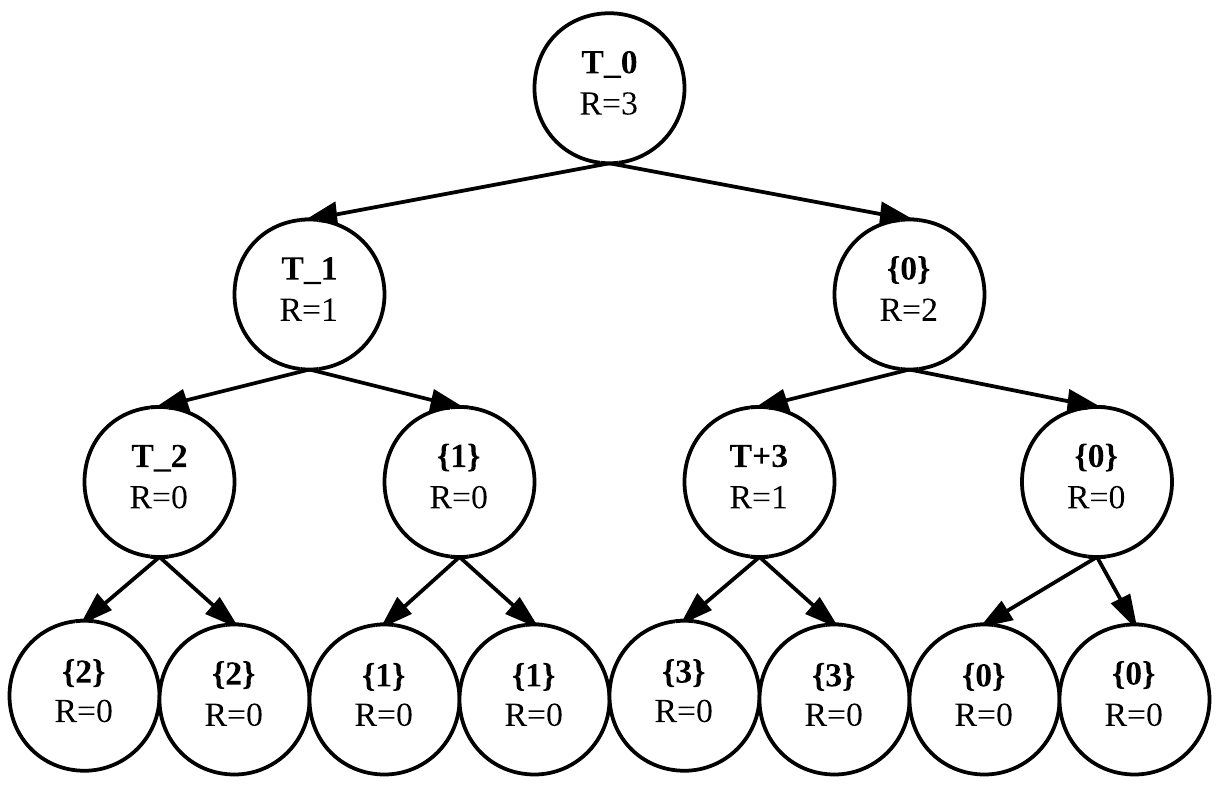
\includegraphics[width=.5\textwidth]{include/mms.png}
\label{mms_thread}
\end{figure}
\linespread{1}
\begin{algorithm*}[t]
\caption{Merge Algorithm}\label{merge}
\begin{algorithmic}
\Require A,B are sorted arrays
\Require length(dst) = length(A) + length(B)

\Procedure{Merge}{$dst, A, B$}
\State $i, j, k\gets0$ \Comment initialize array indicies
\While{(\emph{i within bounds of A) \textbf{and} (j within bounds of B})} 
	\State $dst[k] \gets \textsc{min}(A[i], B[j]$)
		\State \textit{Increment index of array containing min element (i or j)}	
		\State \textit{Increment k}
\EndWhile
\While{(\emph{i within bounds of A)}} \Comment i still in bounds
	\State $dst[k] \gets A[i]$
	\State \textit{Increment i}
\EndWhile

\While{(\emph{j within bounds of j)}} \Comment j still in bounds
	\State $dst[k] \gets A[j]$
	\State \textit{Increment j}
\EndWhile
\EndProcedure
\end{algorithmic}
\end{algorithm*}

\begin{algorithm*}[t]
\caption{MergeSort Algorithm}\label{mergesort}
\begin{algorithmic}[1]
\Require dst and src are arrays of equal length
\Require low and high are indices into A

\Procedure{MergeSort}{$dst, src, low, high$}

\If {$(low < high)$}
\State \emph {pivot} $\gets$ $\textsc{floor}(low+high)/2$
\State \textsc{MergeSort}$(SortedLeft, A, low, pivot )$\Comment sort left half
\State \textsc{MergeSort}$(SortedRight, A, pivot+1, high)$ \Comment sort right half
\State \textsc{Merge}$(dst,SortedLeft, SortedRight)$\Comment merge left \& right

\EndIf
\EndProcedure
\end{algorithmic}
\end{algorithm*}

\begin{algorithm*}[t]
\caption{Multithreaded Mergesort (MMS)}\label{mms}
\begin{algorithmic}[1]
\Require dst and src are arrays of equal length
\Require low and high are indices into src

\Procedure{MMS}{$dst, src, low, high, threads\_remaining$}


	\If{$threads\_remaining == 0$} \Comment perform basic MergeSort
		\State [perform basic MergeSort algorithm] 
	
	\Else \Comment a new thread will be spawned to sort left
	\If {$(low < high)$}
\State \emph {pivot} $\gets$ $\textsc{floor}(low+high)/2$
	\State \emph{t\_left} = $\textsc{Floor}((threads\_remaining-1)/2)$
	\State \emph{t\_right = t\_left}$ + ((threads\_remaining-1)\%2)$
	\State \emph{New\_Thread}$\gets\emph{\textsc{MMS}(SortedLeft,A,low,pivot, t\_left)}$
	\State \emph{\textsc{MMS}$(SortedRight,A,pivot+1, high, t\_right)$}
	\State \emph{\textsc{Wait}(New\_Thread)}
	\State \emph{\textsc{Merge}$(dst,SortedLeft,SortedRight)$}
\EndIf
\EndIf

\EndProcedure
\end{algorithmic}
\end{algorithm*}
 % put this anywhere that is convenient. it uses exactly 1 page

\subsection{Bitonic Sort}
%TODO: Put diagram for this sort.
%TODO: Talk about how data was split for threading.

\section{Testing Framework}
\label{sec:testing}

C++ was selected as the language to implement the testing framework and all the sorting algorithms because of the relative ease and ubiquity of tools to compile for the language. The framework had the following objectives for its design:

\begin{itemize}
\item A common path to benchmark each function to ensure timing is measured consistently.
\item Re-usability of common tasks between the sort algorithms.
\item Common call to a Sort function allow blind usage of sort only passing the number of threads and a vector of data.
\item Ability to swap object that data for sorting was stored in easily.
\end{itemize}

%TODO: Figure
These goals were accomplished through an object oriented set of classes. A common \texttt{SortCommon} class was the parent of all the sort algorithms and contained the means to benchmark an algorithm, generate an unsorted data vector, check if a given set of data is sorted or not, divide set of data using domain decomposition, merging, and padding (used by Bitonic). Each of the sort functions were free to do the sort by any reasonable means necessary. The requirements were that the only two inputs the Sort gets is a set of data and the number of threads it is allowed to divide the data up across. Figure XX shows the layout of these classes and the overall framework.

The algorithm was to sort the data in place (or at least modify the pointer to the new set of data) so that the benchmark function can then validate that the data was sorted. All four of the algorithms did the sort in place (modified the passed in data directly) or created a ``destination'' data set and then swapped the pointer of the two at the end. Memory utilization can become an issue with sets of data this large so copying or making copies of large subsets of the data was not performed in the algorithms.

C++'s \texttt{std::vector} filled with \texttt{unsigned int} was used as the storage object and data type for each of the algorithms. A \texttt{std::vector} is an efficient, dynamically linked list that was selected over an array for the ability to have an easily growing and shrinking memory space (in case an algorithm selected to do an operation involving such a task). We also feel that the C++ compiler can do a better job optimizing the use of a \texttt{std::vector} in our code compared to the relatively manual task of memory management in an array.

The benchmark function prepared a given set of data to pass to the virtual \texttt{Sort} function implemented by each algorithm. The benchmark function also verified that the data was actually sorted when the \texttt{Sort} function returned. The function only ran the timer for a benchmark of an algorithm during the \texttt{Sort} call portion of the testing. This was done to ensure that any overhead tasks performed by the benchmark function itself does not add to the time a given sort runs.

Data could be generated in a few different patterns depending on the type of sort desired for benchmarking. The three options available were a set of data that is actually in order, a set of data that is in complete reverse, and a set of data that was completely random. The first two were used primarily for verification and testing of aspects of the algorithm. The third (random) set of data was used for all testing shown Section~\ref{sec:results} of the report.

The data was checked for sorting using a single-threaded function to look through the elements. The function simply started at the front of the data and moved through all of the elements. If it found an element that was greater than the previous element (in other words, not sorted), the function would multiply the time it took for the sort to run by $-1$ and print a warning stating that the data was not sorted.

A few other other utility functions were also in the \texttt{SortCommon} class. A function that would take the length of the data and how many threads to divide the work amongst would return a \texttt{std::vector} containing a \texttt{std::pair} of the minimum and maximum index for a given thread to perform the sorting on. Bitonic and Quicksort used this in the functional decomposition of the data, but merge used its own algorithm. For bitonic, the data and the number of threads had to be a power of two without modification. A padding and unpadding function is also added to pad zeros to the data in the event the user requests a sort on data that does not meet the power of two requirement for bitonic.

The code was also checked with valgrind to verify that there were minimal memory leaks. Listing~\ref{valgrind} shows the output from valgrind. The listing shows that the code frees everything of concern (definitely lost).

\bashout{valgrind}{Valgrind Output}

GitHub was also used for revision control. This entire project is available for download at \url{http://github.com/jmoles/laser-patroll/}. Doxygen is also commented in-line to generate a set of HTML and PDF documentation for the project.

%TODO: Mention:
% Code having no memory leaks.


\section{Results}
\label{sec:results}
%TODO: Things to mention.
% - Bitonic time with padding if not power of two.
% - Add the four charts that were shown in the presentation.

This section provides the results for the tests of the algorithms. Two different types of tests will be presented. The first is showing the amount of time it took each algorithm to sort with a varying number of threads and constant data size. The other shows the total time all four algorithms took to execute and then percentage of that total time that each algorithm took to run plotting for a constant number of threads and a varying data size.

It is important to note that throughout all of these tests, anything labeled as ``basic'' is \texttt{std::sort} running in a \textbf{serial} fashion. We did not wrap any parallelization around \texttt{std::sort} so that each of the algorithms are evaluated against the sort that would likely be used in C++.

The first series are in Figure~\ref{fig:tvtlg} for a data set of size 134,217,728 elements and Figure~\ref{fig:tvtsm} for a data set of size 512 elements. These tests aimed to see how each algorithm performs with an increasing number of threads both with a small set of data and a large set of data. Ideally, each algorithm should get faster as the number of threads it has available to perform work increases.

% TODO: Why does Quicksort do what it does?
Looking first at the large data set, Merge sort follows the ideal situation quite well and starts to reach a limit in execution time as it gets to the end. Quicksort seems fairly flat over the execution regardless of the number of threads allocated to it. This could be a results of the domain decomposition model of splitting up the work and bringing it back together. As the number of threads increases, there is a final merge that only merges two sets of data at a time. This could result in this final merge occupying more time. 

Bitonic is affected by the same merge issue; however, it has another factor slowing it down. Bitonic shows an average trend of decreasing execution time, but it is susceptible to the requirement that the data and threads must be a power of two. As a result, bitonic performs the best on the situations where the number of threads is a power of two and begins to slow down as it increases from a power of two, peaking one value right before the next power of two.  
%TODO: Small data execution results for size.
%TODO: Single threaded case is missing on the plot.


\begin{figure*}[!t]
  \centering
  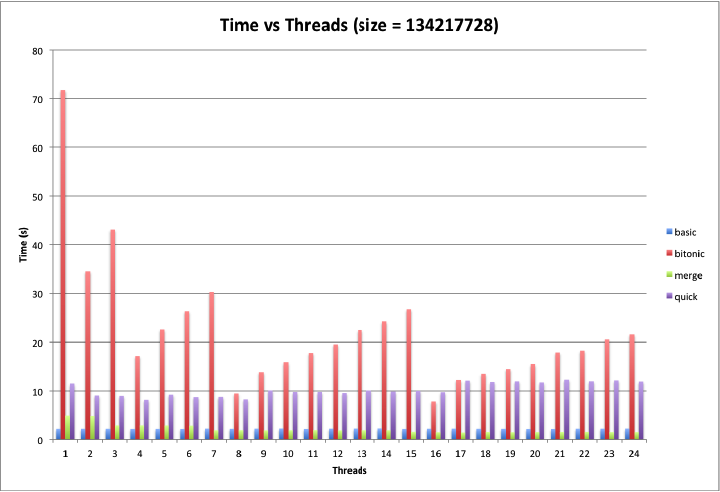
\includegraphics[width=0.7\textwidth]{tvtlg}
  \caption{Time vs Threads Large Data}
  \label{fig:tvtlg}
\end{figure*}

\begin{figure*}[!t]
  \centering
  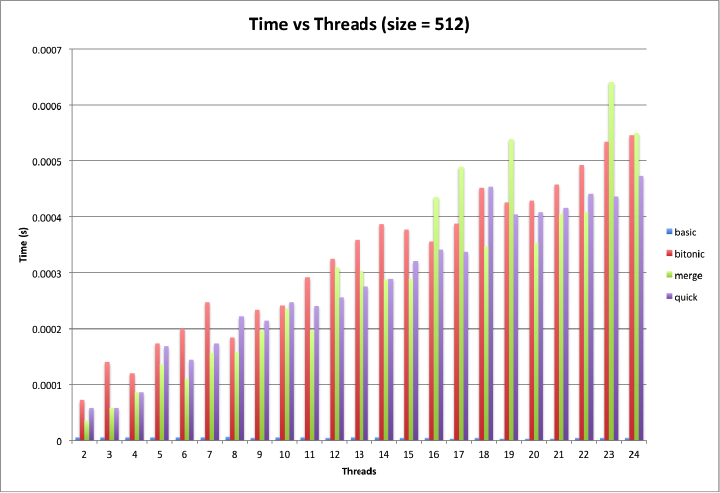
\includegraphics[width=0.7\textwidth]{tvtsm}
  \caption{Time vs Threads Small Data}
  \label{fig:tvtsm}
\end{figure*}

%TOOO/Note: Do these second series even show anything of value? Should we produce something else? Thoughts?

\begin{figure*}[!t]
  \centering
  %\includegraphics[width=2.5in]{myfigure}
  \caption{Time Percentage Four Threads}
  \label{fig:timeperfour}
\end{figure*}

\begin{figure*}[!t]
  \centering
  %\includegraphics[width=2.5in]{myfigure}
  \caption{Time Percentage Twenty Four Threads}
  \label{fig:timepertwentyfour}
\end{figure*}

\subsection{Subsection Heading Here}
Subsection text here.

% needed in second column of first page if using \IEEEpubid
%\IEEEpubidadjcol

\subsubsection{Subsubsection Heading Here}
Subsubsection text here.


% An example of a floating figure using the graphicx package.
% Note that \label must occur AFTER (or within) \caption.
% For figures, \caption should occur after the \includegraphics.
% Note that IEEEtran v1.7 and later has special internal code that
% is designed to preserve the operation of \label within \caption
% even when the captionsoff option is in effect. However, because
% of issues like this, it may be the safest practice to put all your
% \label just after \caption rather than within \caption{}.
%
% Reminder: the "draftcls" or "draftclsnofoot", not "draft", class
% option should be used if it is desired that the figures are to be
% displayed while in draft mode.
%
%\begin{figure}[!t]
%\centering
%\includegraphics[width=2.5in]{myfigure}
% where an .eps filename suffix will be assumed under latex, 
% and a .pdf suffix will be assumed for pdflatex; or what has been declared
% via \DeclareGraphicsExtensions.
%\caption{Simulation Results}
%\label{fig_sim}
%\end{figure}

% Note that IEEE typically puts floats only at the top, even when this
% results in a large percentage of a column being occupied by floats.


% An example of a double column floating figure using two subfigures.
% (The subfig.sty package must be loaded for this to work.)
% The subfigure \label commands are set within each subfloat command, the
% \label for the overall figure must come after \caption.
% \hfil must be used as a separator to get equal spacing.
% The subfigure.sty package works much the same way, except \subfigure is
% used instead of \subfloat.
%
%\begin{figure*}[!t]
%\centerline{\subfloat[Case I]\includegraphics[width=2.5in]{subfigcase1}%
%\label{fig_first_case}}
%\hfil
%\subfloat[Case II]{\includegraphics[width=2.5in]{subfigcase2}%
%\label{fig_second_case}}}
%\caption{Simulation results}
%\label{fig_sim}
%\end{figure*}
%
% Note that often IEEE papers with subfigures do not employ subfigure
% captions (using the optional argument to \subfloat), but instead will
% reference/describe all of them (a), (b), etc., within the main caption.


% An example of a floating table. Note that, for IEEE style tables, the 
% \caption command should come BEFORE the table. Table text will default to
% \footnotesize as IEEE normally uses this smaller font for tables.
% The \label must come after \caption as always.
%
%\begin{table}[!t]
%% increase table row spacing, adjust to taste
%\renewcommand{\arraystretch}{1.3}
% if using array.sty, it might be a good idea to tweak the value of
% \extrarowheight as needed to properly center the text within the cells
%\caption{An Example of a Table}
%\label{table_example}
%\centering
%% Some packages, such as MDW tools, offer better commands for making tables
%% than the plain LaTeX2e tabular which is used here.
%\begin{tabular}{|c||c|}
%\hline
%One & Two\\
%\hline
%Three & Four\\
%\hline
%\end{tabular}
%\end{table}


% Note that IEEE does not put floats in the very first column - or typically
% anywhere on the first page for that matter. Also, in-text middle ("here")
% positioning is not used. Most IEEE journals use top floats exclusively.
% Note that, LaTeX2e, unlike IEEE journals, places footnotes above bottom
% floats. This can be corrected via the \fnbelowfloat command of the
% stfloats package.



\section{Conclusion}
The conclusion goes here.



\section{Lorem}
Lorem ipsum dolor sit amet, consectetur adipiscing elit. Sed nec dictum massa. Phasellus ornare massa congue mi sodales suscipit. Maecenas tristique volutpat porttitor. Quisque venenatis rutrum orci ac auctor. Vestibulum ullamcorper, purus eu tempus malesuada, tellus felis lobortis risus, vel tincidunt felis nunc ut sem. Mauris iaculis tellus non mauris laoreet, sit amet viverra turpis pharetra. Curabitur hendrerit aliquam nunc a elementum. Quisque leo quam, fringilla hendrerit tristique non, consectetur nec elit. Fusce tristique lobortis vestibulum. Nam id dictum libero. Quisque eget lectus commodo nibh egestas consectetur sed vitae elit. Nulla id purus urna.

Etiam hendrerit a diam nec feugiat. Praesent non ultricies est, ac pellentesque neque. Vestibulum eu libero lectus. Vestibulum id justo vitae libero consequat auctor. Mauris et posuere lorem. Etiam sed tincidunt purus. Fusce ac felis arcu. Sed sit amet mi vel enim faucibus porta. Praesent et tincidunt nulla. Nunc tincidunt ligula in lacus posuere, fermentum tempus sapien convallis. Quisque eu lectus fermentum, bibendum dui luctus, aliquet neque. Curabitur a magna fringilla, semper ligula eget, interdum dolor. Etiam aliquet dui sit amet metus faucibus, id tempor metus gravida. Vestibulum nec nibh eu elit imperdiet cursus a sed tortor.

Duis congue fermentum libero vitae feugiat. Quisque vel libero sit amet magna euismod tristique. Sed luctus elit eget sem vehicula consequat. Proin vitae metus erat. Curabitur nisl nisl, ultrices vitae diam faucibus, condimentum volutpat velit. Proin semper nisi nec fringilla aliquet. Pellentesque ante ligula, tempor id placerat vel, tincidunt eget arcu. Sed facilisis accumsan felis, eu scelerisque leo consequat ac. Cras sed pellentesque urna, quis placerat neque. Vivamus rutrum, elit elementum posuere tristique, neque urna imperdiet massa, at interdum velit lorem sit amet neque. Donec fringilla nibh dui, in egestas sapien tempus non. Fusce venenatis, est in gravida dictum, sapien purus sollicitudin dui, eu porttitor nibh sem eu lacus. Mauris quis luctus massa.

Sed luctus turpis nulla, ut faucibus sapien congue id. Vestibulum vestibulum neque vitae luctus consectetur. Nullam tempor non nisi sit amet dictum. Cras auctor semper tortor eget pretium. Ut eu ultrices dolor. Donec ac lectus eget dui semper rhoncus eu et tortor. Nulla eu eros vel turpis imperdiet fermentum ut pretium nisi. Sed eget nunc pretium, consequat nulla in, sagittis massa. Fusce nec dictum tellus. Fusce lobortis erat risus, in fringilla turpis molestie a. Nam commodo nulla leo, vitae semper enim dictum a. Suspendisse a suscipit purus. Quisque in metus at metus aliquet iaculis.

Aliquam fermentum urna sem, at dapibus massa luctus id. Sed sit amet tincidunt nisi. Morbi tincidunt, arcu nec dapibus consequat, est lacus convallis dolor, sed euismod justo purus quis arcu. Vivamus euismod sem erat, in tincidunt sem semper sed. Quisque massa risus, euismod ut neque non, bibendum suscipit quam. Sed eget congue est, sit amet dictum odio. Praesent quam libero, tincidunt non augue sit amet, pellentesque faucibus enim. Integer pellentesque dolor et vulputate pellentesque. Nullam velit nulla, aliquet ac fringilla a, vestibulum non est. In in faucibus felis. Aenean aliquam, neque ac varius volutpat, nulla mauris rutrum mi, ut congue augue justo eu tortor. Nulla eget nisi tempor, sagittis urna eget, iaculis turpis. Nunc malesuada justo mauris, vel tristique magna sodales a. Fusce et massa sit amet urna fringilla interdum. Nulla id augue sit amet sem laoreet iaculis. Nullam id ornare nisl.

Etiam vel urna tellus. Mauris viverra nulla vitae tellus dapibus, sit amet pulvinar nisl luctus. Nunc porttitor diam massa, ut blandit lectus ultrices at. Sed consectetur venenatis turpis interdum ullamcorper. Quisque orci tortor, malesuada vel placerat ac, rutrum non mauris. Phasellus leo neque, venenatis sit amet tellus id, interdum placerat turpis. Mauris ullamcorper volutpat arcu, eu mollis lorem pellentesque elementum.

Integer eget nisl bibendum, tristique turpis vitae, interdum nulla. Quisque sit amet lobortis nulla. Nulla lobortis diam nec luctus aliquet. Suspendisse eleifend sed arcu vitae consequat. Praesent quis ipsum quis nulla varius malesuada. Cras sit amet mi blandit, auctor felis lobortis, feugiat odio. In mattis sodales ligula sit amet porttitor. Quisque quam leo, ullamcorper ut tempus id, venenatis non justo. Suspendisse potenti. Pellentesque dapibus dui sed mauris tristique auctor. Phasellus sed semper nunc. Donec posuere urna ac dictum ultricies. Quisque placerat dui magna, sed faucibus quam posuere sit amet.

Aenean egestas tellus sit amet felis bibendum hendrerit. Aenean eleifend at erat sed mollis. Quisque ac malesuada arcu, id accumsan velit. Morbi a orci ut elit porta eleifend. Fusce metus arcu, sodales vel aliquam eget, semper in odio. Sed fermentum aliquam mauris, ullamcorper auctor ante blandit vitae. Aenean eu massa mauris. Etiam vitae dignissim elit. Phasellus volutpat massa vitae tortor porttitor vestibulum. Pellentesque pulvinar elit sed augue aliquam, in aliquet mauris tristique. Nam eleifend molestie nulla et commodo. Fusce lobortis ligula sed feugiat condimentum. Vestibulum eget tristique arcu. Duis porttitor ac metus vel ullamcorper.

Aliquam dui nibh, egestas et odio quis, auctor tempus dui. Nullam sed convallis nisl. Sed eu vulputate dui. Suspendisse sodales ipsum ut adipiscing suscipit. Phasellus vel diam ornare, placerat lorem quis, posuere odio. Sed id arcu ut ante ultrices laoreet. Sed mattis euismod urna vitae porta. Aenean vel urna eu augue molestie ultricies. Sed molestie ipsum sem, in venenatis nulla facilisis quis. Pellentesque lorem odio, ornare at libero quis, vehicula dignissim nisl. Nam facilisis, elit at mattis vulputate, nisl ipsum molestie purus, ut consequat leo tellus quis diam. Vestibulum volutpat consequat lectus et porta. Phasellus mollis libero quis scelerisque accumsan. Duis a ipsum ultricies, imperdiet nulla tempor, pellentesque arcu.

Proin vel quam feugiat, elementum sem id, vestibulum urna. Pellentesque congue odio at consequat pharetra. Integer quis varius arcu, ac malesuada turpis. In lacus risus, sagittis in arcu at, tincidunt consequat turpis. Ut eget magna accumsan, adipiscing est vel, posuere nunc. Maecenas laoreet aliquam varius. Fusce dictum, sapien tincidunt pretium tempus, lectus nibh fermentum est, sit amet ornare dolor dolor eu nunc.

Aliquam eros quam, lobortis quis faucibus convallis, iaculis bibendum velit. Sed in lectus ut nibh bibendum suscipit id ac justo. Aenean turpis tortor, mollis nec libero id, ultrices hendrerit orci. Nullam eu nulla ut dolor pretium vehicula. Cras auctor nisi vitae eros aliquet, quis pulvinar risus tristique. Praesent nisi arcu, consequat quis tempus quis, porttitor at justo. Curabitur ut mauris vitae massa feugiat congue. Aenean vulputate felis at euismod ultricies. Aliquam at fringilla dui, nec gravida metus. Nunc vulputate bibendum felis ut mollis. Maecenas imperdiet pellentesque erat, quis pellentesque quam venenatis in.

Quisque aliquam ligula felis, vel auctor turpis eleifend eu. Maecenas aliquet quam et magna viverra, et suscipit mi tempus. Fusce sit amet lectus magna. Quisque dignissim porttitor neque, quis accumsan dui gravida et. Sed lacinia quam velit. Duis vehicula neque id aliquam egestas. Phasellus molestie dolor ut posuere convallis.

Donec malesuada ut augue ut mattis. In dictum mauris sapien, eu euismod purus semper in. Nunc malesuada elit erat, vel semper massa gravida et. Proin lobortis auctor condimentum. Vestibulum diam sem, adipiscing et tellus eget, iaculis pellentesque quam. Integer ac nunc eu ipsum ullamcorper blandit vitae ut nisi. Sed commodo magna nec tempor bibendum. Nam metus nisi, malesuada at magna sed, eleifend lobortis massa. Suspendisse facilisis velit vitae malesuada fringilla. Etiam augue massa, aliquam non aliquam ac, vestibulum nec orci.

Vestibulum convallis, eros ut sodales mattis, sapien nisl sodales lectus, vitae blandit lectus mi vel justo. Cras mollis lacinia bibendum. Morbi tristique sem in egestas gravida. Duis hendrerit massa sit amet elit tincidunt, et vestibulum metus condimentum. Donec venenatis luctus est, tempus iaculis orci consequat non. Sed in tortor accumsan urna luctus pulvinar. Nunc velit mi, interdum et turpis eu, porttitor convallis ligula. Curabitur dui augue, commodo sed lacus at, molestie tincidunt enim. In facilisis sapien eget nisi blandit, in fermentum sem viverra. Vestibulum viverra ac lectus vitae vehicula. Quisque condimentum vel mi vitae convallis. Integer convallis suscipit elit a varius. Proin sollicitudin sapien eget nibh cursus viverra. Ut placerat nulla ac nulla suscipit, in posuere enim consequat. Nulla posuere mauris vel ligula eleifend, sit amet condimentum odio pulvinar.

Nullam posuere libero sed lectus ultricies congue. Nam accumsan justo ac ultricies euismod. Cum sociis natoque penatibus et magnis dis parturient montes, nascetur ridiculus mus. Proin leo urna, ultricies quis lacus quis, pulvinar suscipit purus. Cras elementum sed nisl at condimentum. Nulla et porttitor sapien. Proin a gravida leo, vel iaculis turpis. Vivamus lacinia, nunc eu lacinia fermentum, neque felis tempor massa, scelerisque rhoncus lorem quam vitae nulla. Vivamus volutpat erat vitae lacinia congue.

Maecenas scelerisque in ante nec interdum. Integer ullamcorper nulla ac neque iaculis, sit amet semper quam varius. Vivamus sollicitudin imperdiet nunc, sed adipiscing mi. Etiam sed est ipsum. Nullam adipiscing vitae erat nec tincidunt. Donec a tortor sed arcu luctus consectetur. Vivamus viverra mauris eget sollicitudin consectetur.

In aliquet massa in venenatis elementum. Etiam in nibh non leo dictum dignissim. Aliquam in tortor magna. Aliquam dolor nisi, aliquet eu ipsum vel, malesuada volutpat velit. Sed a dui a augue pulvinar ornare id ac urna. Sed fringilla odio at leo rutrum, sit amet imperdiet odio mollis. Nam at velit et sem molestie pellentesque. Curabitur dignissim ipsum fringilla, ullamcorper quam vel, pellentesque dolor. Vivamus imperdiet ultricies mauris, non porta libero pharetra id. Pellentesque vitae sapien sed metus porta elementum non non tellus. Morbi congue tortor turpis, et cursus sapien elementum quis. Duis posuere euismod lacus, quis eleifend urna euismod eget. Aenean sollicitudin odio eget pellentesque luctus. Quisque condimentum, nisi a commodo aliquet, erat arcu tempor nisi, et ullamcorper enim massa ac tortor. Suspendisse porttitor viverra orci sit amet viverra. Donec dolor ipsum, ultrices quis enim eget, molestie imperdiet nisl.

Ut erat velit, auctor quis nulla ac, mattis fermentum leo. Nulla ultrices arcu vitae mattis rutrum. In gravida sapien in dapibus aliquam. Proin luctus mollis dui nec vehicula. Cras ut elit eu mauris luctus lacinia. Vestibulum quis lectus laoreet, tincidunt massa vel, venenatis leo. Aliquam augue tellus, lacinia sit amet nibh ut, dictum rutrum metus. Cras ut risus lorem. Nam eget mi elit. Curabitur eget ipsum enim. Etiam sed iaculis diam, eget fermentum lectus.

Vestibulum quis nunc eget urna lobortis aliquam a id odio. Morbi vehicula dui ac adipiscing suscipit. In hac habitasse platea dictumst. Pellentesque dapibus sagittis erat. Ut fermentum tincidunt volutpat. Integer nec hendrerit erat. Quisque rutrum id elit et vehicula. Vivamus gravida eros rhoncus sollicitudin elementum. In hac habitasse platea dictumst. Curabitur condimentum placerat odio, non feugiat metus vulputate non. Nulla eros leo, aliquet a posuere eget, dictum malesuada lorem. Morbi varius lectus tortor, in tincidunt orci congue in. Ut rhoncus ultricies scelerisque. Phasellus sodales nisi in elit condimentum volutpat. Pellentesque dignissim, orci vitae rhoncus sodales, risus diam rutrum nibh, vitae aliquet ligula urna eu diam. Integer dignissim eros sed dolor pulvinar, non congue elit hendrerit.

Proin tempor adipiscing lobortis. Duis in sapien nibh. Aliquam vel mauris sem. Vestibulum iaculis eleifend neque ac sagittis. Sed quis purus risus. Ut justo purus, vestibulum ac malesuada vitae, pellentesque blandit tellus. Donec elementum turpis ante, vitae dignissim augue tempor eu. Integer gravida erat ut neque fermentum, vel adipiscing mauris consectetur. Cras a ligula lacinia, hendrerit dolor quis, lobortis magna. Sed placerat cursus erat in pretium. Etiam est sapien, cursus interdum interdum dictum, facilisis quis augue. Phasellus feugiat, neque ut placerat facilisis, nunc odio molestie ligula, eu convallis nisl enim sit amet mauris.



% if have a single appendix:
%\appendix[Proof of the Zonklar Equations]
% or
%\appendix  % for no appendix heading
% do not use \section anymore after \appendix, only \section*
% is possibly needed

% use appendices with more than one appendix
% then use \section to start each appendix
% you must declare a \section before using any
% \subsection or using \label (\appendices by itself
% starts a section numbered zero.)
%


\appendices
\section{Proof of the First Zonklar Equation}
Appendix one text goes here.

% you can choose not to have a title for an appendix
% if you want by leaving the argument blank
\section{}
Appendix two text goes here.


% use section* for acknowledgement
\section*{Acknowledgment}


The authors would like to thank...


% Can use something like this to put references on a page
% by themselves when using endfloat and the captionsoff option.
\ifCLASSOPTIONcaptionsoff
  \newpage
\fi



% trigger a \newpage just before the given reference
% number - used to balance the columns on the last page
% adjust value as needed - may need to be readjusted if
% the document is modified later
%\IEEEtriggeratref{8}
% The "triggered" command can be changed if desired:
%\IEEEtriggercmd{\enlargethispage{-5in}}

% references section

% can use a bibliography generated by BibTeX as a .bbl file
% BibTeX documentation can be easily obtained at:
% http://www.ctan.org/tex-archive/biblio/bibtex/contrib/doc/
% The IEEEtran BibTeX style support page is at:
% http://www.michaelshell.org/tex/ieeetran/bibtex/
\bibliographystyle{IEEEtran}
% argument is your BibTeX string definitions and bibliography database(s)
%\bibliography{IEEEabrv,../bib/paper}
\bibliography{IEEEabrv,mendeleysources,manualsources}
%
% <OR> manually copy in the resultant .bbl file
% set second argument of \begin to the number of references
% (used to reserve space for the reference number labels box)


% biography section
% 
% If you have an EPS/PDF photo (graphicx package needed) extra braces are
% needed around the contents of the optional argument to biography to prevent
% the LaTeX parser from getting confused when it sees the complicated
% \includegraphics command within an optional argument. (You could create
% your own custom macro containing the \includegraphics command to make things
% simpler here.)
%\begin{biography}[{\includegraphics[width=1in,height=1.25in,clip,keepaspectratio]{mshell}}]{Michael Shell}
% or if you just want to reserve a space for a photo:

\begin{IEEEbiography}{Eric Krause}
%TODO: Type Eric's contribution.
bio
\end{IEEEbiography}

% if you will not have a photo at all:
\begin{IEEEbiography}{Josh Moles}
%TODO: Type Josh's Bio
Biography text here.
\end{IEEEbiography}

% insert where needed to balance the two columns on the last page with
% biographies
%\newpage

\begin{IEEEbiography}{Erik Rhodes}
%TODO: Erik's bio
bio
\end{IEEEbiography}

% You can push biographies down or up by placing
% a \vfill before or after them. The appropriate
% use of \vfill depends on what kind of text is
% on the last page and whether or not the columns
% are being equalized.

%\vfill

% Can be used to pull up biographies so that the bottom of the last one
% is flush with the other column.
%\enlargethispage{-5in}



% that's all folks
\end{document}


